\chapter{Evolutionary modeling of the differential contribution of Neanderthal ancestry to complex traits provides insights into selective forces that shape trait variation}
\section{Introduction}
We recently developed a methodology to assess whether Neanderthal ancestry is over- or under-represented in the genetic component of complex phenotypes compared to random genetic variation. Based on 500,000 individuals from the UK Biobank, we found the estimated contribution of Neanderthal alleles (NIMs) to phenotypic variation (NIM heritability) is significantly depleted in the great majority of the phenotypes. This is consistent with the observation that in general, natural selection has acted to remove Neanderthal alleles since introgression. On the other hand, we have found that Neanderthal alleles were significantly over-represented in their contribution to a handful of traits.
To understand the evolutionary models that could explain these observations, we performed forward-in-time population genetic simulations to model the evolution of Neanderthal and non-Neanderthal alleles according to a demographic model relating modern humans and Neanderthals. We chose parameters used in a previous study (Petr PNAS 2019) analyzing the fitness cost of Neanderthal introgression. Specifically, an ancestral population of size 10,000 diploid individuals splits into a human population and a Neanderthal population, each one evolves separately before a single pulse of Neanderthal admixture followed by subsequent random mating. Under this demography, we modeled evolution of phenotypes subject to different forces including directional, stabilizing, and disruptive selection. We estimated a NIM heritability Z-score, a measure of whether NIM heritability deviates significantly from the background alleles. We found under most models of selection, the NIM heritability Z-score is near zero or negative, indicating NIM heritability is neutral or depleted. Interestingly, we were able to recreate a positive NIM heritability Z-score, indicating an elevated Neanderthal contribution to heritability in two separate models of stabilizing and directional selection. In the stabilizing selection model, the optimal value of the trait is decreased in the human branch during the split between humans and Neanderthals leading to a positive NIM heritability Z-score. We also observe a positive NIM heritability Z-score in a directional selection model in which the parameter that couples SNP effect size and fitness is reduced after introgression. This observation highlights possible mechanisms for how complex traits evolved in human history by examining the genetic contribution of Neanderthal ancestry.
\section{Results}
Our goal was to examine how different evolutionary models affect NIMs and their contribution to phenotypic heritability. Specifically we sought to determine if variants of Neanderthal ancestry contribute to an enriched amount of heritability (NIM heritability) compared to a background set of MAF and LD matching SNPS under different conditions.To determine this we ran population genetic simulations to model evolution of phenotypes under several evolutionary forces including directional, stabilizing, and disruptive selection. 
\subsection{Examining how models of stabilizing, directional and disruptive selection impact NIM heritability}
We first created a simple demographic model to quickly test different types of selection \ref{fig:5.1}. We used forward-in-time simulation software SLiM 3.0 \cite{haller2019slim} in order to create a demographic model of a common ancestral population followed by a split between Neanderthals and modern humans and finally a single pulse of introgression. Using this model, we were able to simulate how selective forces impacted evolution of polygenic phenotypes by looking at the quantitative trait loci (QTLs). We then examined the QTLs in order to quantify how they were affecting heritability of a phenotype.
We first examined how the evolutionary force of stabilizing selection impacted heritability in our simple demographic model. Under the force of stabilizing selection extreme values of a phenotype are not favored, while there is an optimum value of said quantitative phenotype. We used a model of stabilizing selection developed by Lande et. al. \cite{lande1976natural} in which each phenotype ($y$) has an optimum value ($\omega$) which would impact fitness ($f$) (Fig \ref{fig:5.2}). We then ran our forward in time simulations under the simple demographic model and examined the QTLs to see how they would impact heritability in modern humans. We partitioned the QTLs into those of Neanderthal ancestry (NIMs) or those not of neanderthal ancestry (\textit{see chapter 3 for full definition}). We calculated heritability of NIMs and compared them to a matching background set matched by MAF and LD to determine enrichment of NIM heritability. Under this model of stabilizing selection, we were not able to see any significant change in NIM heritability (\textit{as defined in chapter 3}).
We then examined how directional selection impacts NIM heritability in our simple demography. We used a 
    -stabilizing lande 1976
    -directional eyre walker
    -disruptive zeng
- modified the selection
    -stabilizing with an optimum shift
    -directional with varying tau parameter
- made complex demographic simulations
- testing other paramters
    -different effective population sizes
    -effect on different genomic element sizes
    -different admixture proportions
    -different causal proportions 
\section{Methods}
\subsection{Simple demographic model – stabilizing selection}
In order to test our 
\newpage
\section{Figures}
\begin{figure}[htb]
    \centering
    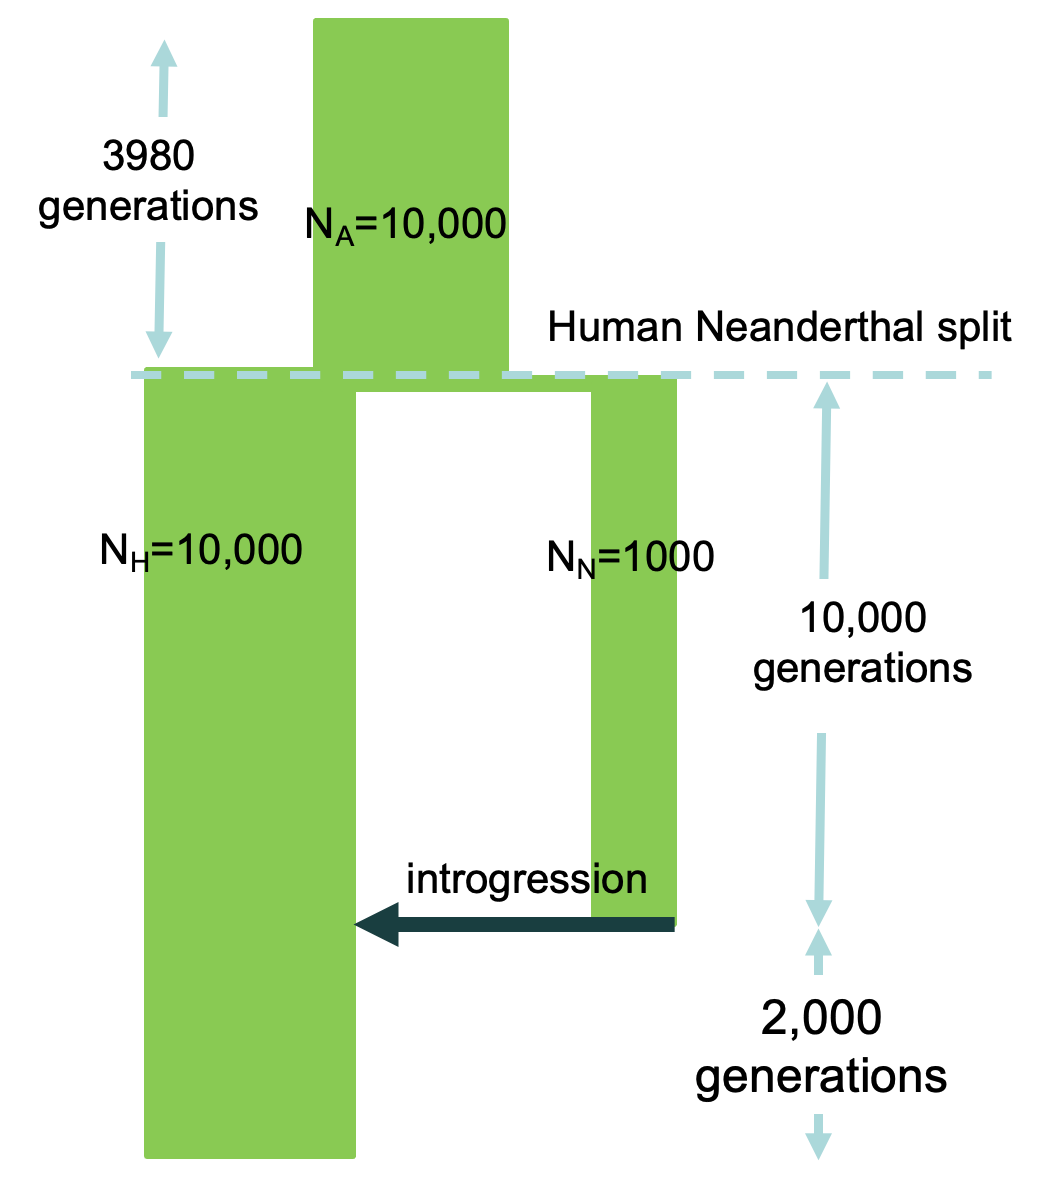
\includegraphics[width=\textwidth]{chapter5/figures/fig5.1.png}
    \caption{Caption}
    \label{fig:5.1}
\end{figure}

\begin{figure}[htb]
    \centering
    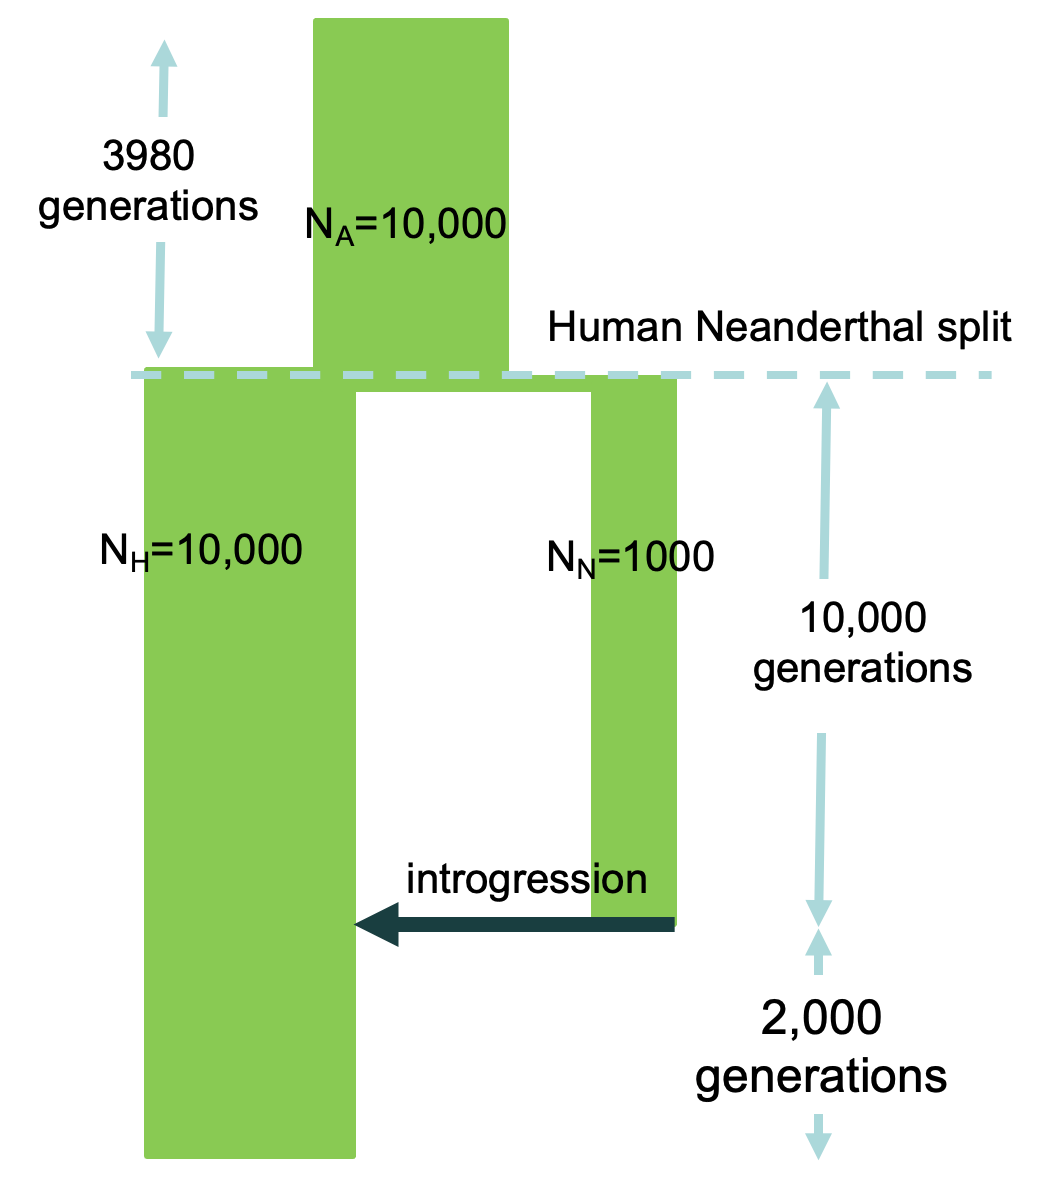
\includegraphics[width=\textwidth]{chapter5/figures/fig5.2.png}
    \caption{Caption}
    \label{fig:5.2}
\end{figure}

\begin{figure}[htb]
    \centering
    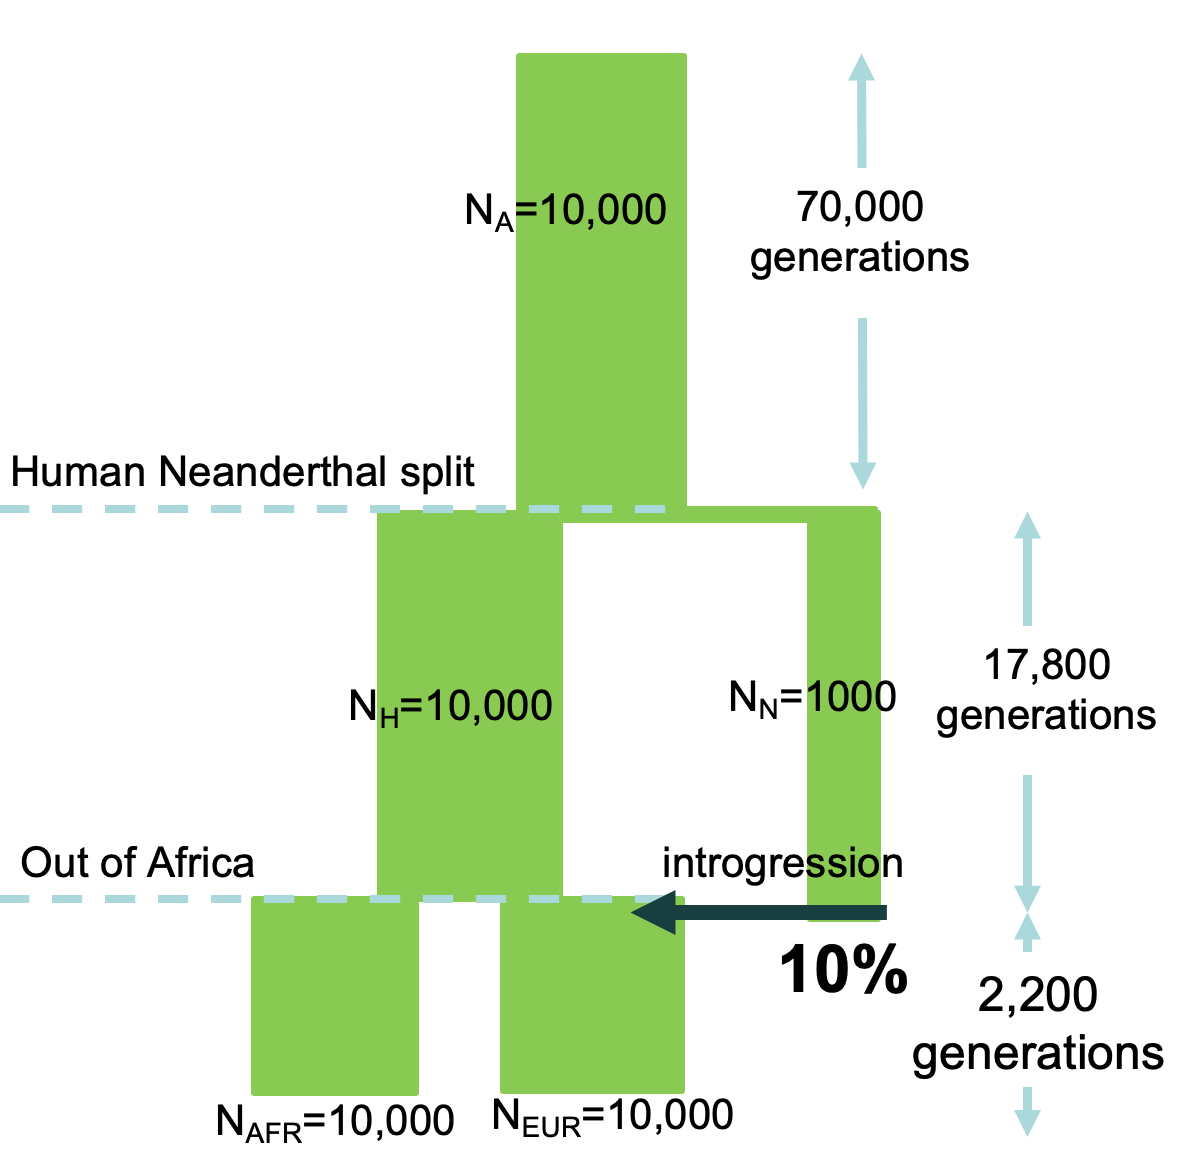
\includegraphics[width=\textwidth]{chapter5/figures/fig5.3.png}
    \caption{Caption}
    \label{fig:5.3}
\end{figure}

\begin{figure}[htb]
    \centering
    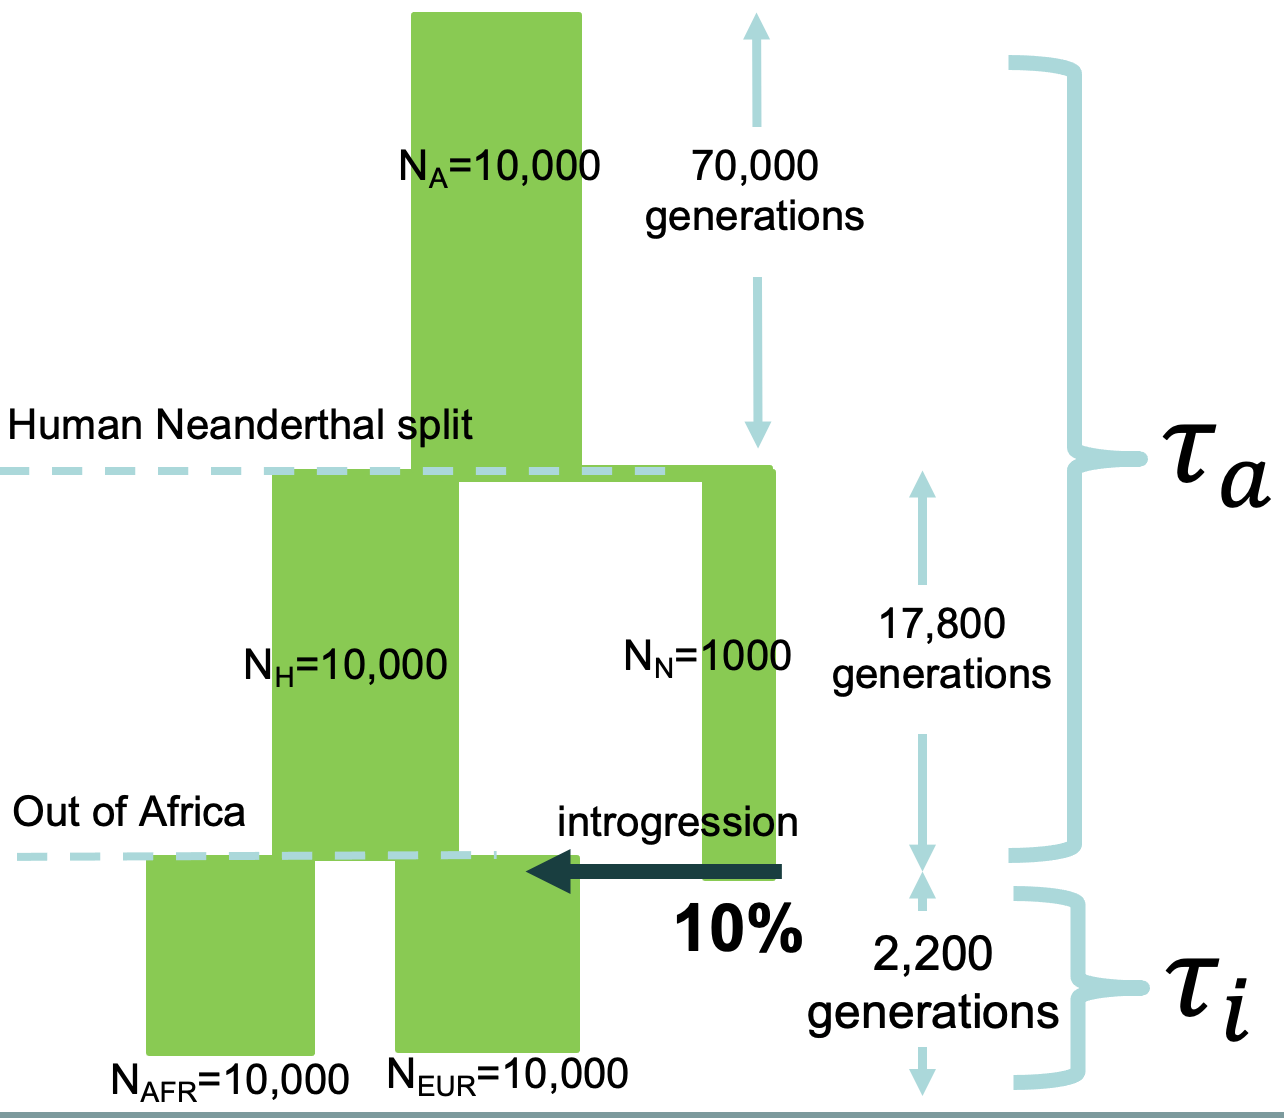
\includegraphics[width=\textwidth]{chapter5/figures/fig5.4.png}
    \caption{Caption}
    \label{fig:5.4}
\end{figure}